\documentclass[10pt,twocolumn]{article}
	
\usepackage{myfontstyle}
\usepackage{mypackages}
\usepackage{mymacros}
\usepackage{mycommands}

\begin{document}
\thispagestyle{fancy1}

%%% Title and Abstract------------------------
\twocolumn[
\begin{center}
	\hrule
	\vspace{3pt}
	% Title:
	{\sffamily\bfseries\Large
		Report for Laboratory Two: Voltage Dividers
	} \\
	{\color{gray}
		\vspace{3pt}
		\hrule
		\vspace{3pt}
	}
	{
		\hspace*{\fill}
		Austin Piper
		\hspace*{\fill}
		Alex Blakley
		\hspace*{\fill}
		Ahmed Irfan
		\hspace*{\fill}
%		Fourth Author    % uncomment these two lines if there's a fourth author
%		\hspace*{\fill}
	}\\
	\vspace{3pt}
	{\itshape
		\hspace*{\fill}
		Department of Mechanical Engineering, Saint Martin's University
		\hspace*{\fill} \\
		\hspace*{\fill}
		ME/EE 316---Mechatronics \& Measurements Laboratory
		\hspace*{\fill}
	}\\
	\vspace{3pt}
	{
		\hspace*{\fill}
		\today{} % today's date ... can type manually instead
		\hspace*{\fill}
	}
	\vspace{3pt}
	{\color{gray}\hrule}
%	\vspace{2pt}
\end{center}
% Abstract:
\begin{adjustwidth}{1.5in}{1.5in}
{\small
\noindent\textbf{Abstract.} \hspace{1em}
	Applying a 10V DC power supply to a voltage divider circuit with two resistors in series, the voltage across both resistors remains constant while the voltage across a single resistor changes depending on the resistance. Using a myRIO  configured with the labVIEW software to change our input voltage and measure the voltage source and the resistor voltage. When connecting a arbitrary function generator to an oscilloscope, a variety of wave functions at 5Vpp had a period of 2.5ms.
}
\end{adjustwidth}
\vspace{9pt}
\hrule
\vspace{1\baselineskip}
]

%%% Body -------------------------


\section{Introduction} 
\label{sec:introduction}

	
(\autoref{sec:results}). 

\section{Materials and Methods}

	This lab has three parts. In the first part of the lab two resistors were placed in series on a bread board connected to a DC power supply set to 10V. Using a multimeter measure the voltage across each resistor and both resistors. Then replacing the second resistor and taking measurements again for all four different resistors. 
	
	\begin{figure}
	\centering
	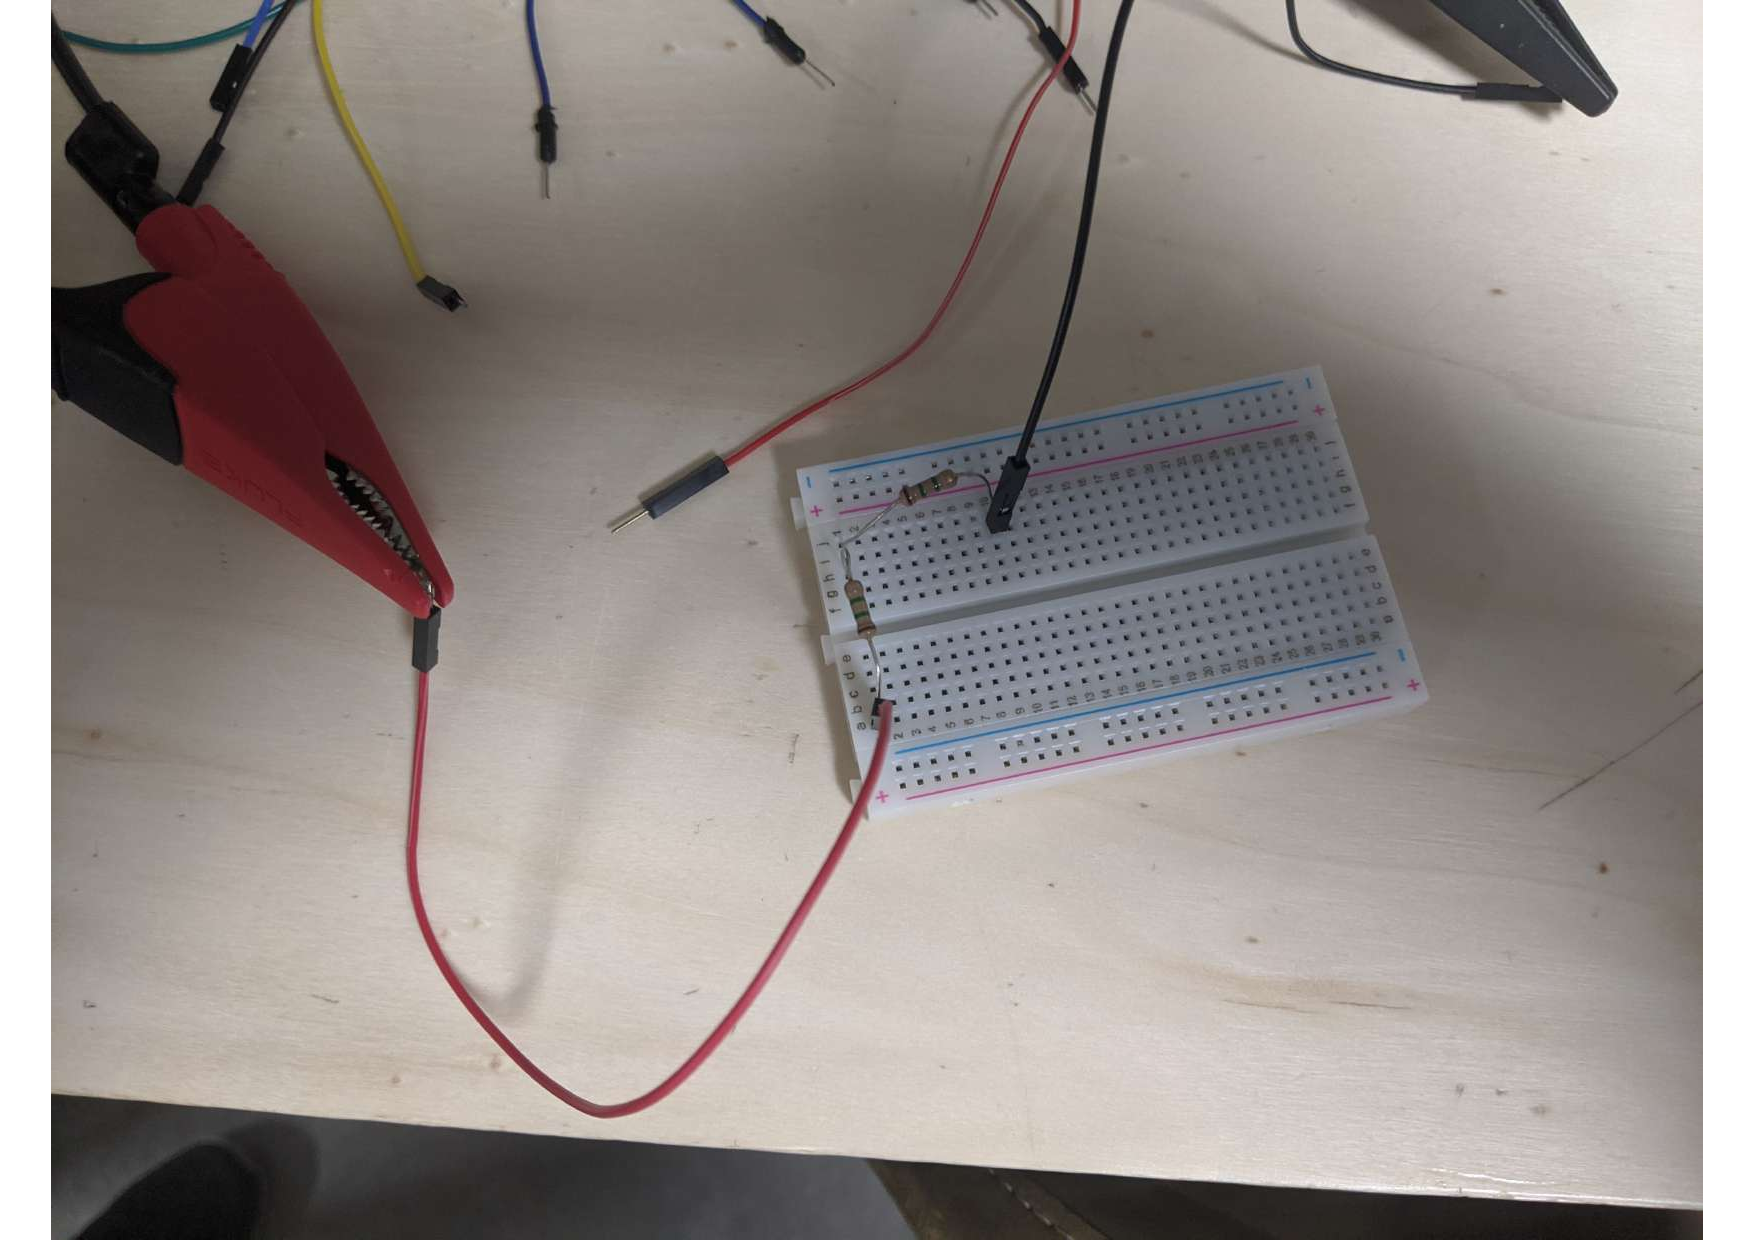
\includegraphics[width=.9\linewidth]{figures/vdc.pdf}
	\caption{Voltage divider circuit}
	\label{fig:circuit}
\end{figure}

	For part two of this lab a myRIO configured with the labVIEW software was be used as the power supply and measurement tool, on the same voltage divider circuit. The myRIO was connected to measure the voltage across both resistors and the voltage across the second resistor. Using labVIEW an analog output and input were made to recieve data from the myRIO, as well as a voltage vs time chart window. Starting at 0V and working up to 10V, in increments of 1V, the voltage source and the resistor voltage is displayed in labVIEW and recorded.Again replacing the second resistor with each of the different resistors and repeating measurements. 
	
	\begin{figure}
	\centering
	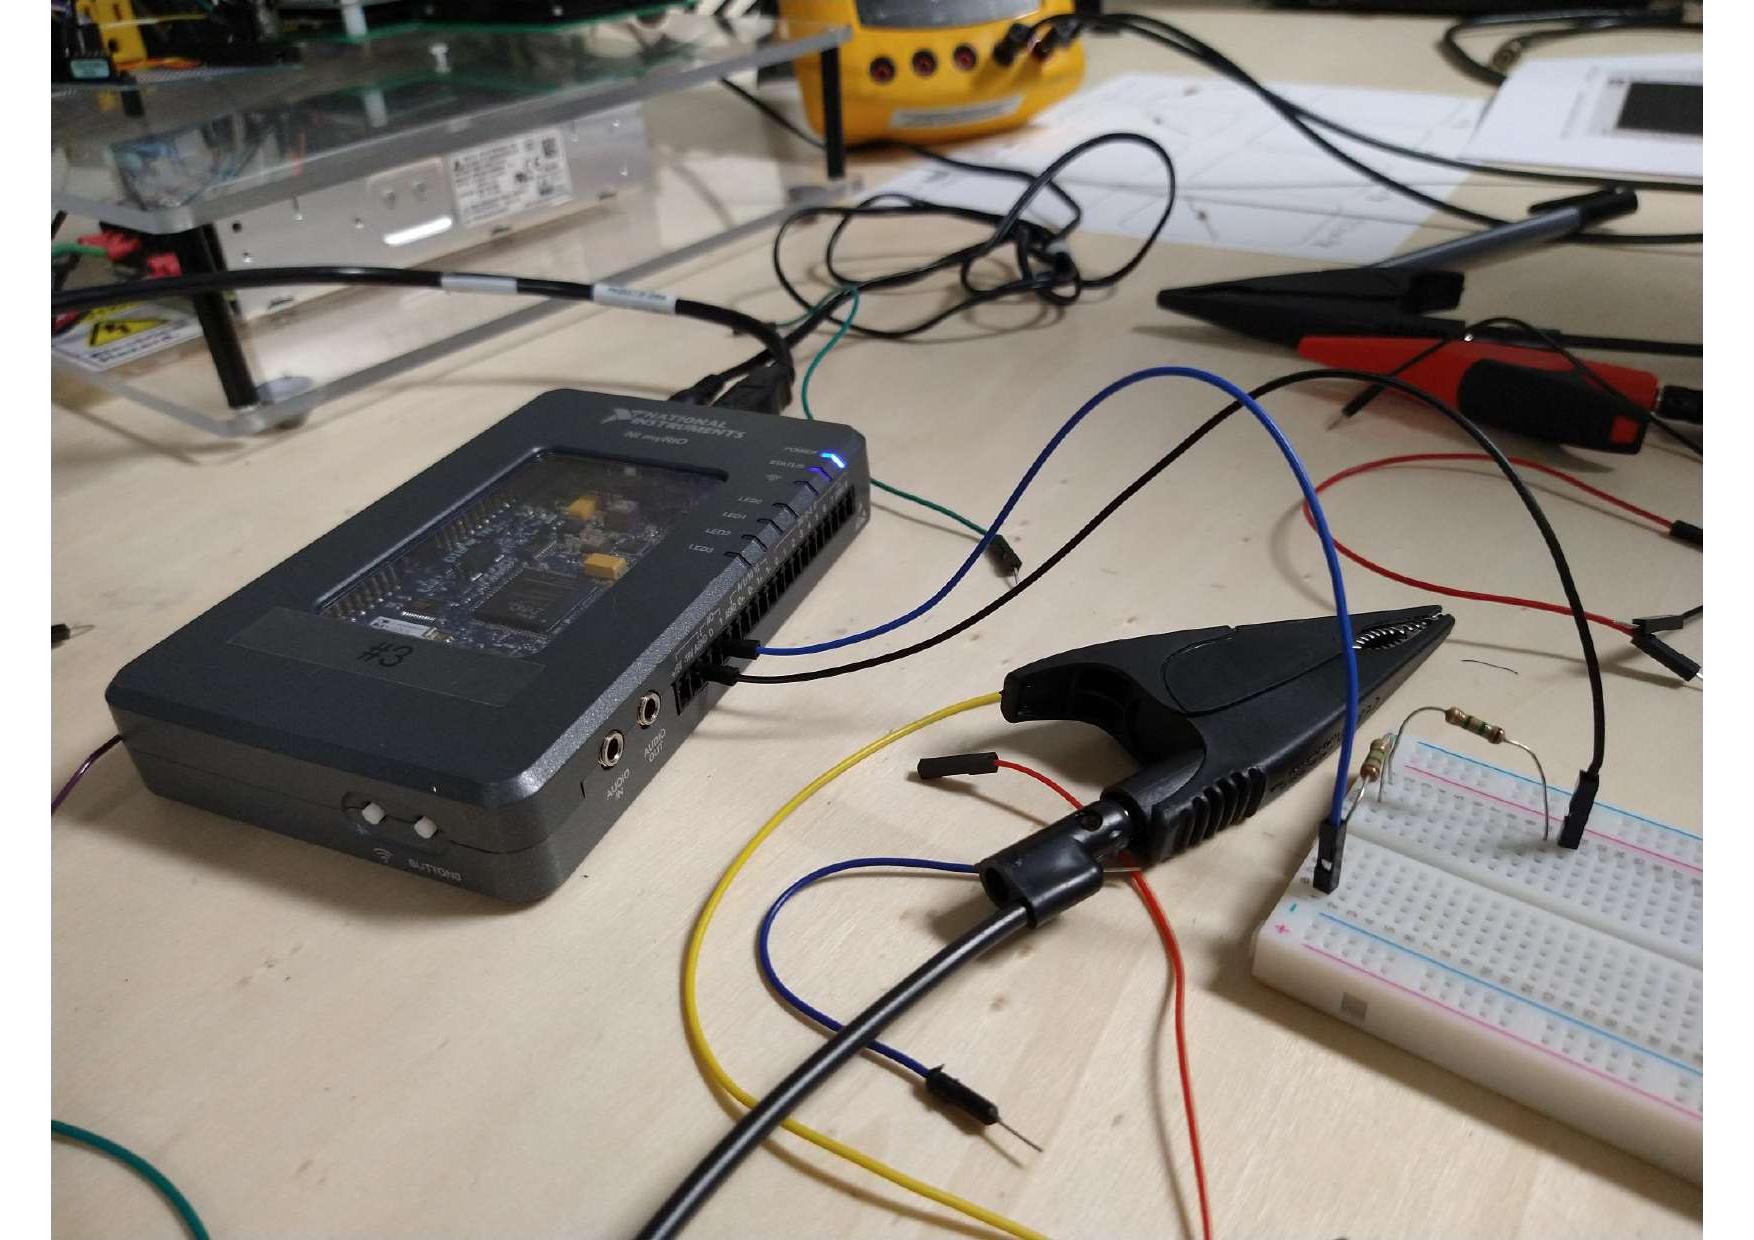
\includegraphics[width=.9\linewidth]{figures/myr.pdf}
	\caption{myRIO Voltage divider circuit}
	\label{fig:circuit2}
\end{figure}




\begin{enumerate}
\item 

\item 

\item

\end{enumerate}






\section{Discussion}

``This is the section of the paper for you to show off your understanding of the data. You should summarize what you found. Explain how this relates to what others have found. Explain the implications.''

\section{Author Contributions}



%%% References -------------------------

\bibliographystyle{plainnat}
\bibliography{report}

%%% Appendices -------------------------

\appendix

\section{Appendix: \LaTeX{} Tutorial}\label{sec:latex}



\subsection{Equations}



\begin{subequations}
\begin{align*}
	x &= 2 y & \text{(where $x>2$)} \\
	y &= 4 x + 8 &
\end{align*}
\end{subequations}


\subsection{Figures}


\begin{figure}[bt]
	\centering
	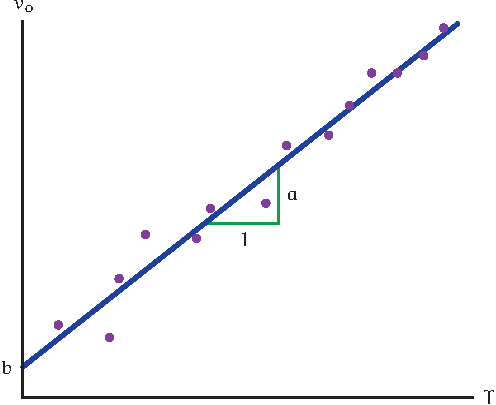
\includegraphics[width=.9\linewidth]{figures/data.pdf}
	\caption{here's a caption.}
	\label{fig:data}
\end{figure}



\subsection{Tables}

 
\begin{table}[bt]
	\begin{tabularx}{1\linewidth}{ lXX }
		
	\end{tabularx}
	\caption{a table caption.}
	\label{tab:dummy}
\end{table}


\end{document}  
